\documentclass[12pt]{article}
\usepackage[english]{babel}
\usepackage{amsmath,amsthm}
\usepackage{graphicx}
\usepackage{caption}
\usepackage{subcaption}
\usepackage{amsfonts}
\usepackage{indentfirst}
\usepackage{lscape}
\usepackage[top=2.5cm,bottom=2.5cm,right=2.5cm,left=2.5cm]{geometry}
\usepackage{titlesec}
\setcounter{secnumdepth}{5}

% ----------------------------------------------------------------
\begin{document}

\section{Quantification}

The Quantification is the step we will use for determine which images correspond to which species. For that we will use the bag of words in a first place to simplify the signature of whole images. And after use the K-nn method for the classification.

\subsection{Bag of words}

In the bag of words method we found two different step, the calculation of K-means and the design of a signature for the images.

\subsubsection{K-means}

The K-means is a simply method which consist to reduce the number of points or vectors in our case. The first step is to determinate randomly k centroid vectors, after with an Euclidean distance \eqref{euclid} we attribute the descriptors to whole images to the nearest centroid vectors.

\begin{equation}
\sum_{k=0}^{centroid}\sum_{i=0}^{desc}\parallel x_k - u_i \parallel ^2
\label{euclid}
\end{equation}

The last stage is an update step, for each centroid vectors we calculate the means of whole the descriptors associate to, so we obtain a new centroid vectors. And we applicate this algorithm for x iteration choose by the user.

For an application on a cloud of points we obtain this kind of result:



\subsubsection{Signature}

The creation of the signature is the last step of the bag of words method, they consist to assign to each images a signature in function of the number of word in the image. The graphic representation of this signature is a histogram: 

\begin{figure}[h]
        \centering
        \begin{subfigure}[b]{0.5\textwidth}
                \centering
                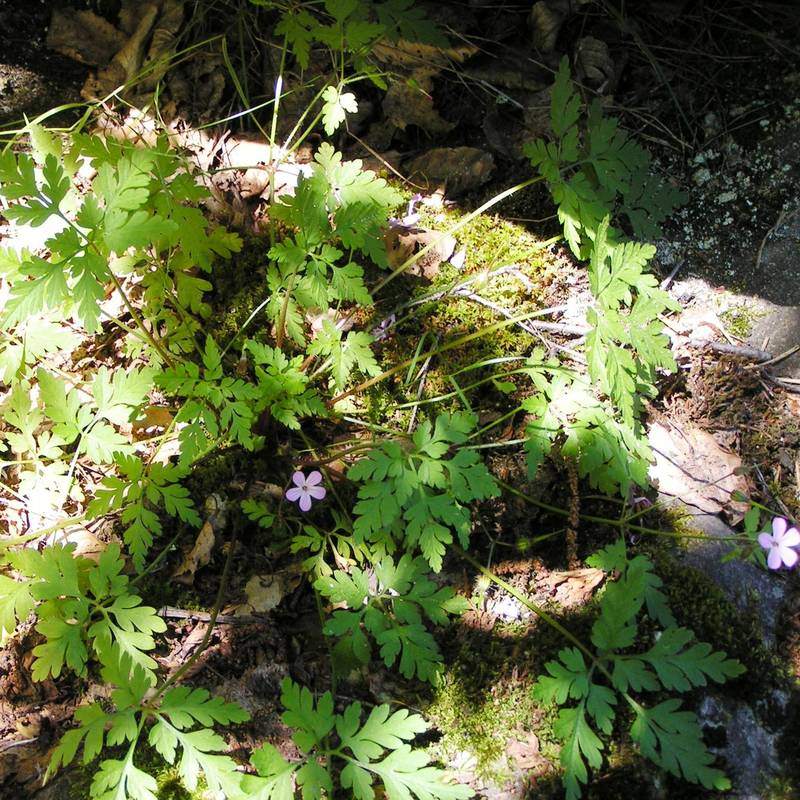
\includegraphics[height=180px]{128.jpg}
        \end{subfigure}%
        \hfill
        \begin{subfigure}[b]{0.5\textwidth}
                \centering
                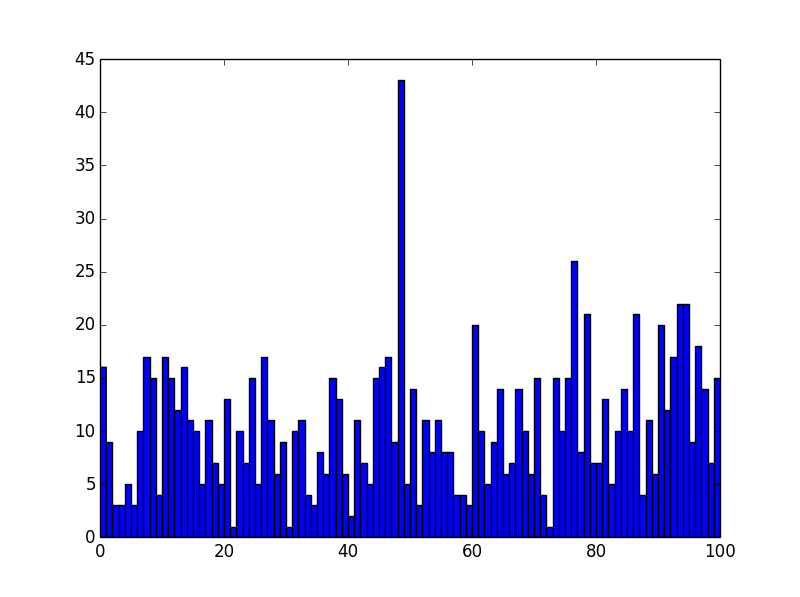
\includegraphics[height=180px]{128_sig.png}
        \end{subfigure}
        \caption{Signature de l'image 128}
        \label{fig:signature1}
\end{figure}

\begin{figure}[h]
        \centering
        \begin{subfigure}[b]{0.5\textwidth}
                \centering
                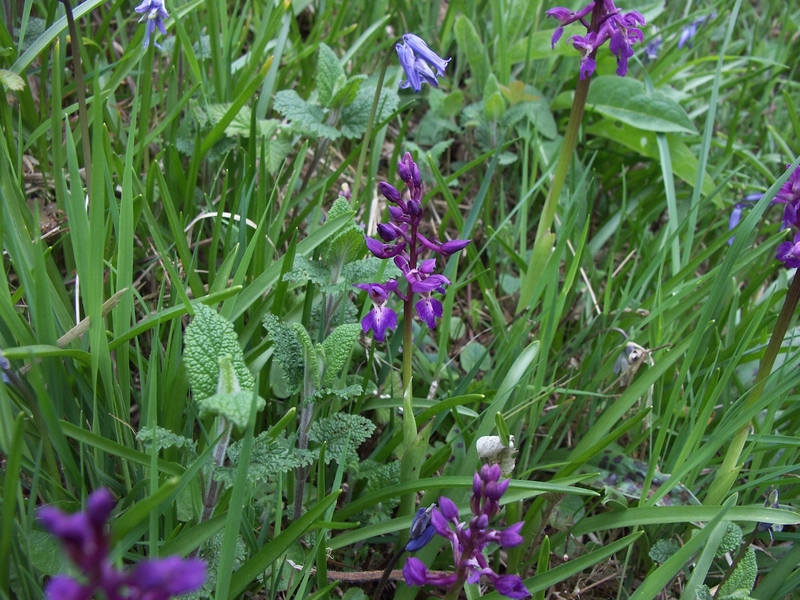
\includegraphics[height=180px]{132.jpg}
        \end{subfigure}%
        \hfill
        \begin{subfigure}[b]{0.5\textwidth}
                \centering
                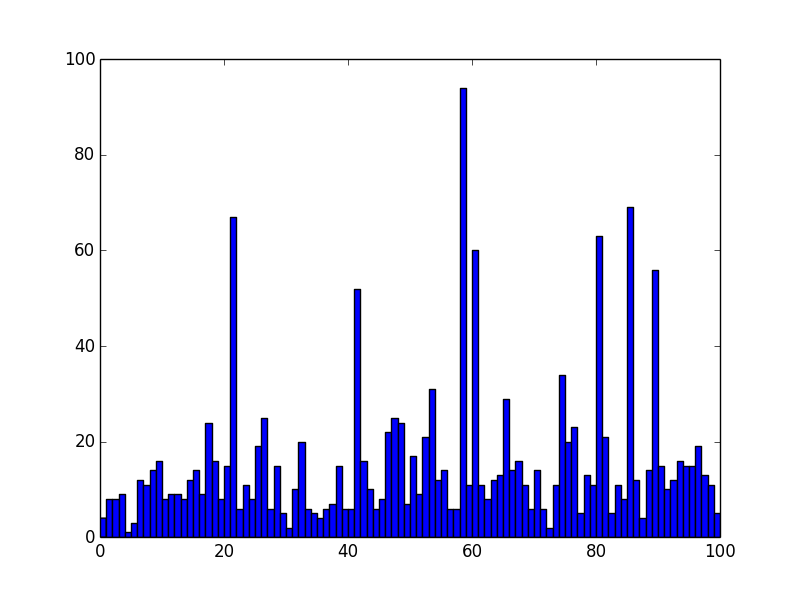
\includegraphics[height=180px]{132_sig.png}
        \end{subfigure}
        \caption{Signature de l'image 132}
        \label{fig:signature1}
\end{figure}

\subsection{K-nn}

% ----------------------------------------------------------------
\end{document} 